\documentclass{FR16} 
\usepackage{listings}
\usepackage{pdfpages}
\usepackage{subfiles} 


\begin{document}

\maketitle

% ML template reports
% https://www.cs.utexas.edu/~mooney/cs391L/paper-template.html
%https://github.com/udacity/machine-learning/blob/master/projects/capstone/report-example-1.pdf
\newpage
\tableofcontents
\newpage
\listoffigures
\newpage
\section{Abstract}
The aim of the project is to analyse, develop prediction models and define data clusters from the "New York City Airbnb Open Data" from a Kaggle competition.
\\ In particular, one part is focused on the development of predictive models to forecast house prices using these Supervised Learning technics:\begin{itemize}
\itemsep0em 
\item Linear Regression
\item Decision Tree
\item Random Forest
\item Ranger Random Forest
\item Neural Newtworks
\end{itemize}
For each of these, a comparison between the Mean Square Error and between all $R^2$ measure of all methods has been made to highlight which have the best performance. Also, for training all the models, a partition of the dataset in three parts has been applied: entire dataset, filtered by neighboorhood group and filtered for neighboorhood group and room type. In this way, it is possible to check the perfomance giving less or more features in input.\\\\
The second part is focused on the cluster and data reduction technics using these Unsupervised Learning technics:
\begin{itemize}
\itemsep0em
\item K-means Algorithm 
\item Clustering for mixed-type data
\item Principal Component Analysis
\end{itemize}

%%Eachreport must contain:\\
%•shortabstract: what are your going to present %in the report\\
%•statementof the problem/goalof the analysis %and description of thedata set(s)\\
%•list of three to fivefindings/keypoints\\
%•the analysis with wisecommentary\\
%•(optional) theoretical background of the used %methods\\
%•conclusions(should include the findings/%keypoints)\\
%•theAppendix, containing all the R codeNotice:
%\\•Thepaper lengthisirrelevant provided that %the content is correct.
%\\•No R code in the main text.The R code must %be confined to the appendix\\
%•The report should be prepared inPDFonly

\newpage
\section{Problem Definition and Algorithm}
\subsection{Two main Goals}

\subsubsection{Develop predictive models for price}
The first objective is the forecast of the prices given some input information. This could be usefull for a lot of scenarios. For example from a AirBnB customer point of view, he/she would like to get the list of houses more in alignment with his/her preference choice; or for a host point of view, where given the position and other information he/she could get information about the possible per day price of his property in New York City. 

\subsubsection{Define clusters and groups}
The second objective is the definition of group or partition between the houses with different characteristics. For a user point of view could be usefull to have information about avaiable houses similar to those booked in the past. This could be also usefull after the booking for a suggestion analysis having the information about last booked houses in NewYork or houses in similar cities around the world.
\newpage
\subsection{Algorithms}
\subsubsection{Linear Regression}
 Linear regression  is a linear approach to modeling the relationship between a dependent variable and one or more independent variables. 
 
  \subsubsection{Decison Trees}
In decision analysis, a decision tree can be used to visually and explicitly represent decisions and decision making.

 \subsubsection{Random Forest}
 Random forests are an ensemble learning method for classification, regression and other tasks that operate by constructing a multitude of decision trees.
 \subsubsection{Ranger Random Forest}
Ranger is a fast implementation of random forests or recursive partitioning, particularly suited for high dimensional data. 

\subsubsection{Neural Networks}
Neural networks are a set of algorithms, modeled loosely after the human brain, that are designed to recognize patterns.

\subsubsection{K-means}
K-means is a method of vector quantization, originally from signal processing, that aims to partition n observations into k clusters in which each observation belongs to the cluster with the nearest mean.

\subsubsection{Principal Component Analysis}
Principal Component Analysis (PCA) is mostly used as a tool in exploratory data analysis and for making predictive models.

\newpage
\section{Experimental Evaluation}

\subsection{Methodology}
\subsubsection{Data Inspection}
The dataset is part of a Kaggle competition, called the New York City Airbnb Open Data. It contains 48.000 rows per 16 columns.
The dataset is structured with these columns: 
\begin{itemize}
\itemsep0em 
\item \textbf{id}
\item \textbf{name}: name of the listing
\item \textbf{host\_id}
\item \textbf{host\_name}
\item \textbf{neighbourhood\_group}: location
\item \textbf{neighbourhood}: area
\item \textbf{latitude}: coordinates
\item \textbf{longitude}: coordinates
\item \textbf{room\_type}: space type
\item \textbf{price}:  in dollars
\item \textbf{minimum\_nights}: amount of nights minimum
\item \textbf{number\_of\_reviews}: number of reviews
\item \textbf{last\_review}: latest review
\item \textbf{reviews\_per\_month}: number of reviews per month
\item \textbf{calculated\_host\_listings\_count}: amount of listing per host
\item  \textbf{availability\_365}: number of days when listing is available for booking\\
\end{itemize}
It has been select only 5 of these variables: price, latitude, longitude, neighbourhood\_group and room\_type. The reason is that it is reasonable to select them to predict the prices and to obtain different clusters. The position and the neighbourhood is important since if a property is positioned near the city center will have a higher price with respect to those situated in the outskirts; also the type of room, since an entire apartment will cost more than a single room. \\\\
From the Figure \ref{fig:1} is possible to see the distribution of the price. The minimum price is $0$ and the maximum is $10000\$$. It is not possible to rent a house for free, so it is possible to filter the price with a price higher than $15\$$. It is possible that a luxury house cost a lot per day, but these value can not be consider in the model, instead they are outliers and for this reason it is convenient to filter the price again and take those that have a value lowert than $500\$$. The reason is that the third quantile has a price of $175\$$ which is a far from $10000\$$ (Figure \ref{fig:3}). It has also been checked the null and missing value  in the dataset and has not been found apart from the reviews\_per\_month column. It is not a problem, since this feature has been not taken in account to train the models. 
\\
\begin{figure}[H]
\centering
\includegraphics[width=0.3\textwidth]{figures/figure1.jpg} 
\caption{\label{fig:1}Price summary}
\end{figure}
\noindent From Figure \ref{fig:2}, it is possible to see the distribution of all houses in New York City and the price. This picture is not really informative since it can be noticed that the prices for the most part are in the range $0$-$500\$$ and only a low number of istances have a price greater than $500\$$. Deleting the outliers, the Figure \ref{fig:3} is more informative than the one before.

\begin{figure}[H]
\centering
\includegraphics[width=0.5\textwidth]{figures/figure2.pdf} 
\caption{\label{fig:2}Distribution of all houses in NY colored by prices}
\end{figure}

\begin{figure}[H]
\centering
\includegraphics[width=0.5\textwidth]{figures/figure3.pdf} 
\caption{\label{fig:3} Distribution of all houses in NY of price between $15\$$ and $500\$$ per day}
\end{figure}
\subsubsection{Data Cleaning and Pre-processing}

The dataset has approximately 48.000 rows for each column, so an important part of the work is related to the pre-processing due to the large amount of data. For this reason, some variable has been rescaled to let the models to learn faster and better and to perform a better prediction. Latitude and longitude have not been rescaled for forecast price model, while for clustering methods to have a consistent distance calculation. Categorical variables have also been rescaled assigning a numerical value to each category, resulting as unordered factors.\\
The selected categorical variables are: neighbourhood\_group and room type.\\
The selected numerical variables are: latitude, longitude and price.
\\\\
Considering that every neighbourhood group has his characteristic, also taking in account the room type that could impact largerly the price. It is possible to define of different subset of the original set and try different methods of forecast. This is due to the fact that a customer should choose which of the different neighbourhood and room type is interested in. Models have been run to different scenarios (Figure \ref{fig:4}): users interested in all New York City houses and all type of room, users interested only in a single neighbourhood and users interested in a single neighbourhood and a single room type. 
\\ Including different scenario could be potentially computationally expensive. In reality, the training proceeded without any problem. \footnote{ The models have been trained on a machine with quad-core 3.5 GHz processor, 8 Gb RAM and 4 Gb dedicated GPU.} Computantional problem may emerge for the case of hyperparametrisation tuning, even using multiprocessing and multithreading technics. For semplicity, in this project no model tuning have been made. \\
Also for clustering have been filter every scenario, but not for the case of Hierarchical Clustering because it need to generate a readable dendogram using the mean of all neighbourhood or room type price, Principal Component Analysis since avaiable data are really small for some specific neighbourhood like Staten Island and specific room type.


\begin{figure}[H]
\centering
\includegraphics[width=0.5\textwidth]{figures/figure4.PNG} 
\caption{\label{fig:4}  Approximated distribution map of all houses in Manhattan }
\end{figure}



\subsection{Results}

\begin{figure}[H]
\centering
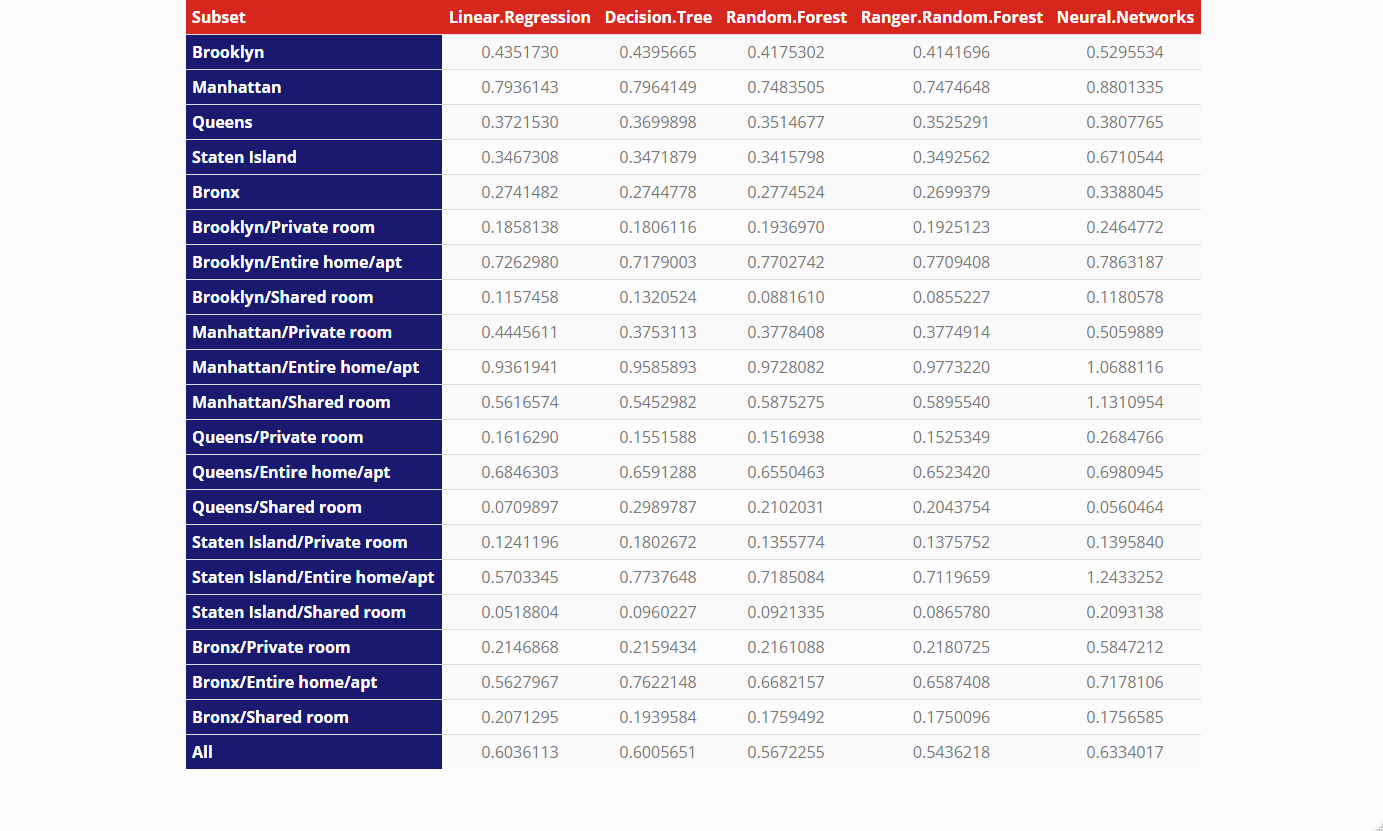
\includegraphics[width=1\textwidth]{figures/model_summary.PNG} 
\caption{\label{fig:5} Summary of the MSE for all the models for each subset of the dataset }
\end{figure}

\subsubsection{Linear Regression Results}
For the Linear regression the model give different results based on the variables used. \\\\
\textbf{Linear Regression selecting the Neighboorhood group}\\
For semplicity, the tests have been only taken filtering for Manhattan data points, but changing the neighboorhood the results are similar. 
Results are acceptable (Figure 5), given a $R^2$ value of $0.4011$ and a Mean Square Error, comparing prediction and test set, of $0.67$.
\\\\ \textbf{Linear Regression selecting the Neighboorhood group and the type of room}\\
As in the previous case the tests are for Manhattan and for Entire home/Aparment type of room.\\
The model output (Figure 6) a value of $R^2$ equals to $ 0.05953$ which is low  and a Mean Square Error, comparing prediction and test, of $1.23$.
\\\\ \textbf{Linear Regression without filters}\\
The model (Figure 7) obtain a $R^2$ value of $0.4031$ which is acceptable and a Mean Square Error, comparing prediction and test set, of $ 0.59$.
\begin{figure}[H]
\centering
\includegraphics[width=0.5\textwidth]{figures/lm2.PNG} 
\caption{\label{fig:6}  Linear Regression output filtering by  Manhattan}
\end{figure}
\begin{figure}[H]
\centering
\includegraphics[width=0.5\textwidth]{figures/lm3.PNG} 
\caption{\label{fig:7}  Linear Regression output filtering by  Manhattan and Entire home/Apartment }
\end{figure}
\begin{figure}[H]
\centering
\includegraphics[width=0.5\textwidth]{figures/lm1.PNG} 
\caption{\label{fig:8} Linear Regression output without filters }
\end{figure}



\begin{center}
\begin{tabular}{l  c c }
\arrayrulecolor{Azzurro}
\hline
{\bfseries Linear Regression
} & MSE & $R^2$  \\
\hline
{\bfseries Entire dataset} & 0.59 & .40  \\
{\bfseries Filter: Mahnattan} & 0.76 & 0.355  \\
{\bfseries Filter: Manhattan \& Apt} & 0.44 &  0.12  \\
\hline
\end{tabular}
\end{center}


\subsubsection{Decison Trees Results}
For the Decision tree the model give different results based on the variables used.
\\\\ \textbf{Decison tree  without filters}\\
\\\\
\textbf{Decison tree selecting the Neighboorhood group}\\
\\\\ 
\textbf{Decison tree  selecting the Neighboorhood group and room type}



\begin{center}
\begin{tabular}{l c c c }
\arrayrulecolor{Azzurro}
\hline
{\bfseries Decision Tree
} & MSE & $R^2$  \\
\hline
{\bfseries Entire dataset} & 0.59 & ..  \\
{\bfseries Filter: Mahnattan} & 0.77 & ..  \\
{\bfseries Filter: Manhattan \& Apt} &  0.40 & ..  \\
\hline
\end{tabular}
\end{center}
\subsubsection{Random Forest Results}
There were no problem running Random Forest regression for the price, givin the default parameters. For the parameter tuning there were no possibilities for the entire dataset, due to the large number of data points. For the filtered dataset, instead, were possible to tune the mtry, number of maximum nodes and number of trees.
\\\\ \textbf{Random Forest  without filters}\\
There were no possibility to run a forecast of the price
\\\\
\textbf{Random Forest selecting the Neighboorhood group}\\
\\\\ 
\textbf{Random Forest selecting the Neighboorhood group and room type}
Using the tuning of the parameter the results are slightly better. The model start with a $23\%$ explained variance to a value of $25\%$.


\begin{center}
\begin{tabular}{l c c c }
\arrayrulecolor{Azzurro}
\hline
{\bfseries Random Forest
} & MSE & $\% Var $  \\
\hline
{\bfseries Entire dataset} &  0.56 & 43.9   \\
{\bfseries Filter: Mahnattan}& 0.70 & 38.9   \\
{\bfseries Filter: Manhattan \& Apt}&  0.38 & 21.6   \\
\hline
\end{tabular}
\end{center}
\subsubsection{Ranger Random Forest Results}
Ranger Random Forest is known to be computationally light with respect to the classic Random Forest. In fact, for the tuning part there were not problem in running it for the entire dataset. 
\\\\ \textbf{Ranger without filters}\\
Ranger outputs for the entire dataset are consistent. We have a $R^2$ of 0.47 and OOB error of .
\\\\
\textbf{Ranger selecting the Neighboorhood group}\\
The dataset filtered by Neighboorhood ouputs a value of 0.4 $R^2$ and a OOB error of.
\\\\ 
\textbf{Ranger selecting the Neighboorhood group and room type}
The dataset filtered by neighboorhood and room type gives as result a $R^2$ of 0.25.
\\\\


\begin{center}
\begin{tabular}{l c c c }
\arrayrulecolor{Azzurro}
\hline
{\bfseries Ranger RF
} & MSE & $\% Var $ \\
\hline
{\bfseries Entire dataset}& 0.53 & 46.6 \\
{\bfseries Filter: Mahnattan} & 0.71 &  38.8  \\
{\bfseries Filter: Manhattan \& Apt}& 0.38 & 21.7   \\
\hline
\end{tabular}
\end{center}



\subsubsection{Neural Network Results}


\begin{center}
\begin{tabular}{l c c c }
\arrayrulecolor{Azzurro}
\hline
{\bfseries  Neural Networks
} MSE & Loss \\
\hline
{\bfseries Entire dataset} & 0.61 &  0.53 \\
{\bfseries Filter: Mahnattan} & 0.84  & 0.64 \\
{\bfseries Filter: Manhattan \& Apt} & 0.48 & 0.44  \\
\hline
\end{tabular}
\end{center}

\subsubsection{K-means Results}


\subsubsection{Principal Component Analysis Results}

\newpage
\subsection{Discussion}

\subsubsection{Linear Regression Discussion}
Linear regression model gives interesting results for the non-filtered dataset and also for the filtered by neighbourhood group.
All variable results to rejected by Null hyphotesis, so the model depends on all the selected variables.
Latitude and longitude are correlated with the target, room type is strongly positive correlated with the price and neighbourhood group does not seem to have
a great contribution in the prediction of the price.
\\

\subsubsection{Decision Tree Discussion}
The performance with respect to the other models are not the best, but acceptable. The predicton results are not also very precised for the filtered neighboorhood 
and room type. Also, the plots of the predicted value are not so consistent since the values are divided in category which correspond to the leaves that are not so strong
with respect to the other model predictions.
\\

\subsubsection{Random Forest Discussion}
Random forest outputs consistent results and performs  better than linear regression and decision tree. 
Parameters tuning does not give big improvement in performance and also are computationally expensive.
\\

\subsubsection{Ranger Random Forest Discussion}
Results of Ranger are the best with respect to the previous models. Also the tuning part was fast and computationally cheaper than 
the classic Random Forest model but does not give great improvements in performance.
\\
\subsubsection{Neural Network Discussion}
\subsubsection{K-Means Discussion}
\subsubsection{Principal Component Analysis Discussion}

\section{Conclusion}

From the result the method with the most higher accuracy is the Random Forest method... while the worst are ....
\\Moreover, Random Forest method is also the worst in term of computation time for the tuning part since it takes for a configuration with 4 core, more or less 1 hour to tune the parameters. 

\
\subsection{Linear Regression}


\subsection{Decision Tree}
Decision  tree are one of the most used model in the Machine Learning world since are very familiar to human users and can be easily plotted. 
\\



\subsection{Random Forest}
Random Forest is an ensemble method which use a combination of decision tree to get the prediction.
\subsubsection{Ranger Random Forest}
Ranger Random Forest is a computationally light model which results are very close the classical Random Forest.
\\





\newpage
\section{Appendix}
%\subfile{project}


%\includepdf[pages=-, pagecommand=\thispagestyle{plain}]{project.tex}
%\noinden

\newpage


\subsection{Footnote}
You can create a footnote like this.\footnote{I created a footnote.}



\newpage
\begin{thebibliography}{9}
\bibitem{giusti}
Giusti, Santochi, \emph{Tecnologia Meccanica e Studi di Fabbricazione}. Casa Editrice Ambrosiana, Seconda Edizione
\bibitem{mechteacher}
Mechteacher, \emph{Knuckle Joint – Introduction, Parts and Applications},\\ http://mechteacher.com/knuckle-joint/
\bibitem{totalmateria}
Totalmateria, \emph{G32NiCrMo8}, http://www.totalmateria.com 
\bibitem{sandvik}
Sandvik Coromant,\emph{Catalogo  generale  2018},   http://www.coromant.sandvik.com/it
\bibitem{uni}
Norme UNI, Ente nazionale italiano di unificazione
\end{thebibliography}

\end{document}